\chapter{Experiments}
\label{chap:experiments}

In this chapter the experiments and experimental results of this work are displayed. First we establish the general experimental setup. Afterwards the results of the conducted MVTecAD LOCO \cite{LOCODentsAndScratchesBergmann2022}
survey are presented in section \ref{sec:locoxperiments}. As a baseline for performance evaluation we uitilize the performance on the more conventional MVTecAD dataset \cite{MVTEC_Bergmann_2021}, 
as well as a classifier comparison. In section \ref{sec:faltconnectorxperiments} we review the performance of the classifiers on our novel dataset category. Lastly section \ref{sec:ensembleresults} 
deals with the findings regarding the ensemble network approach, also conducted on the MVTecAD LOCO dataset and the new dataset category introduced in this work.


\section{Experimental Setup}
\label{sec:experimentsetup}

All models trainings and result reproductions have been conducted on the IAD cluster student partition. The GPU in use for all nodes used by that partition (ist die formulierung gut?) is and 
RTX 2080Ti with 11GB of memory, and the CPU is an AMD Ryzen 9 16-Core processor. The cluster overview \cite{clusterdocs} serves to provide further detail for additional questions. As for software, 
pytorch 2.1.2 was utilized to implement the ensemble model. The specifications of other libraries, as well as the specifications for the MVTecAD LOCO experiment are documented in the 
environment files in the project code.



\section{MVTecAD LOCO Experiments}
\label{sec:locoxperiments}

In this section we review the performance of the IAD methods mentioned in section \ref{sec:IADmethods} on the MVTecAD LOCO \cite{LOCODentsAndScratchesBergmann2022} 
dataset. Tables xyz, xyz, and xyz each display the experiments with regards to one of the metrics: image AUROC, pixel AUROC and sPRO. \newline
Comparing the average image and pixel AUROCs to the ones reported in the chapter \ref{chap:background} a decrease in performance is visible. 
This is also true in regards to the pixel wise AUROC on average. (noch hinschreiben welche classifier den maximalen drop off hatten und 
welche den wenigsten hatten). (Schreiben Welche classifier on average die besten waren für jede metric)

- image auroc Tabelle hier hin

Investigating the column wise performance, the classes of the dataset seem to have varying challenge levels. Albeit some fluctuations, 
the juice bottle class seems to be consistently getting very high results in image and pixel AUROC, especially regarding the latter. 
Conversely, the class screw seems to often have lower image AUROC resuts.

- pixel auroc hier hin


The sPRO values calculated for the approaches were of poor performance as seen in table xyz. Despite this, comparing the metrics to the 
class averages reportet in \cite{LOCODentsAndScratchesBergmann2022}, the results seem legitimate. Bergmann et al. review several methods 
in this paper that they selected to be applicable on logical anomalies. The lowest scoring models were often barely above some metrics reportet 
below, if at all. (Beschreiben wer so gute ansätze sind bei sPRO on average)

- sPRO tabelle hier hin

Figure xyz shows exemplary metrics divided by structural and logical anomalies. Here a better performance is clearly visible for the 
class of structural anomalies, suggesting logical anomalies to be distinctively more difficult to corregtly predict and segment.

- bild mit logical vs anomalous hier hin

Additionally below in figure xyz are exemplary images from multiple classes that showcase good and bad segmentation results. 

- Figure mit segmentation results



\begin{figure}[htbp]
    \captionsetup[subfigure]{justification=centering}
    \centering
    \begin{subfigure}[b]{0.3\textwidth}
        \centering
        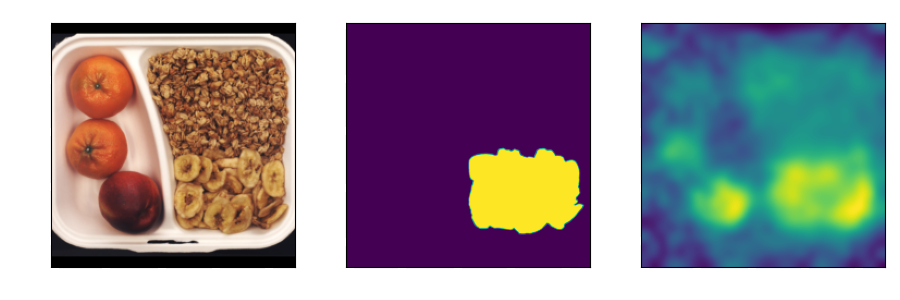
\includegraphics[width=\textwidth]{figures/locopatchcoreresults/breakfast_box_test_logical_anomalies_003.png}
        %\caption*{Logical Anomalies}

    \end{subfigure}
    \begin{subfigure}[b]{0.3\textwidth}
        \centering
        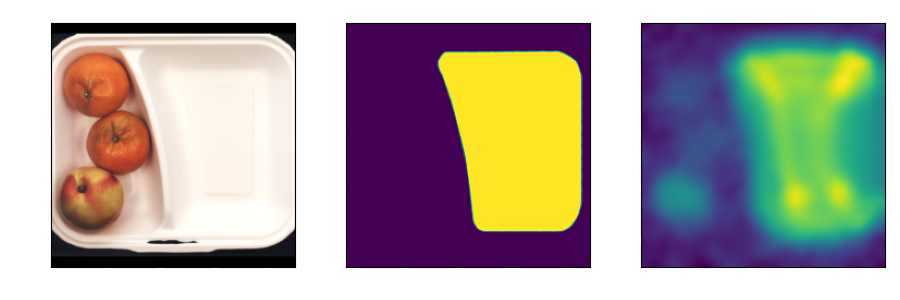
\includegraphics[width=\textwidth]{figures/locopatchcoreresults/breakfast_box_test_logical_anomalies_034.png}


    \end{subfigure}
    \begin{subfigure}[b]{0.3\textwidth}
        \centering
        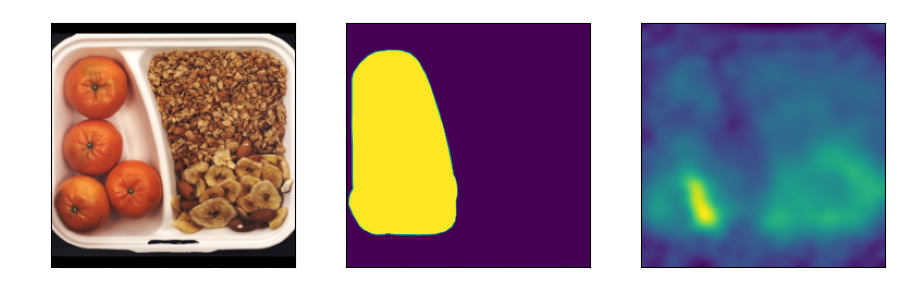
\includegraphics[width=\textwidth]{figures/locopatchcoreresults/breakfast_box_test_logical_anomalies_070.png}


    \end{subfigure}
    \begin{subfigure}[b]{0.3\textwidth}
        \centering
        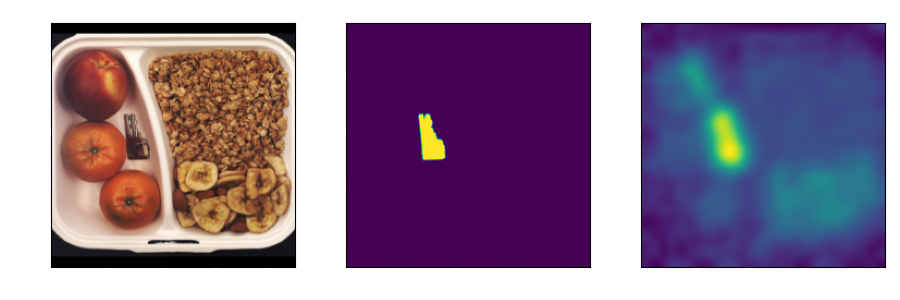
\includegraphics[width=\textwidth]{figures/locopatchcoreresults/breakfast_box_test_structural_anomalies_014.png}
        %\caption*{Structural Anomalies}

    \end{subfigure}
    \begin{subfigure}[b]{0.3\textwidth}
        \centering
        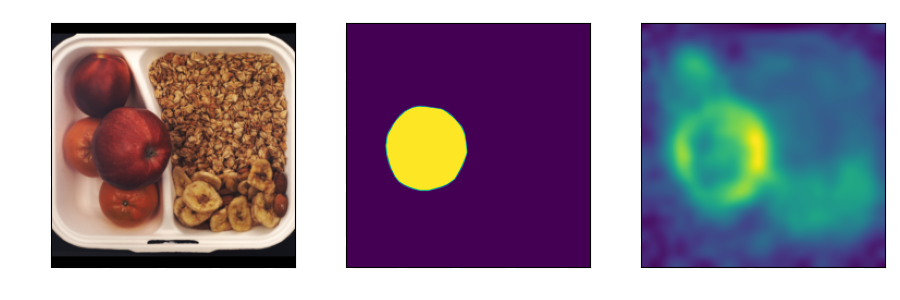
\includegraphics[width=\textwidth]{figures/locopatchcoreresults/breakfast_box_test_structural_anomalies_024.png}


    \end{subfigure}
    \begin{subfigure}[b]{0.3\textwidth}
        \centering
        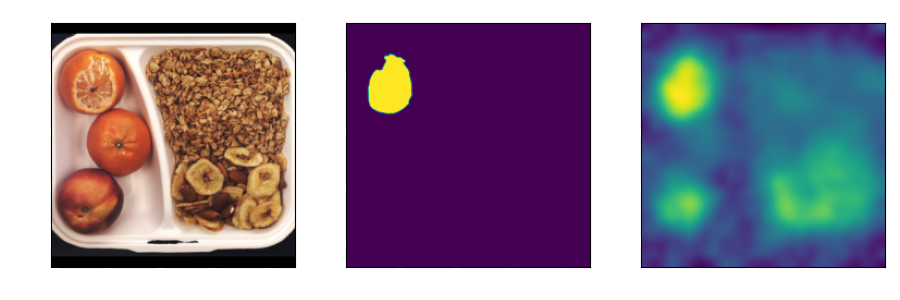
\includegraphics[width=\textwidth]{figures/locopatchcoreresults/breakfast_box_test_structural_anomalies_070.png}


    \end{subfigure}
    \caption{Exemplary Results of PatchCore on the Breakfast Box Class}
    \label{fig:PCBB}
\end{figure}

\section{Flat Connector Experiments}
\label{sec:faltconnectorxperiments}

- same analysis like last section\newline
- analyse performance from 5 classifiers, ensemble performance is for next section


\section{Ensemble Network}
\label{sec:ensembleresults}

This section reports the results of the ensemble network approach on the class flat connector to facilitate understanding of a visual 
analyis. More results from other classes of the MVTecAD LOCO \cite{LOCODentsAndScratchesBergmann2022} set are to be found in appendix (referenz). Conclusions drawn from this 
experiment are also applicable to the other classes. Firstly the results from the primary ensemble approach from section \ref{sec:featurelevelensemble} are reported. Afterwards 
the results of the secondary ensemble approach are presented, supported by according metrics and segmentation examples.


\subsection{Independent Transformation Block}
\label{subsec:ITBfail}

When performing the ensemble training process using the approach by \cite{EnsembleHeller2023}, the results were generally not usable. Looking at the exemplary plot of the segmentation 
results in figure \ref{fig:pca_res}, it becomes obvious why no metrics are reported for this experiment. When investigating image level metrics, they were highly inconsistent thorughout 
the training process and are regarded as not meaningful and representative.

\begin{figure}[htbp]
    \captionsetup[subfigure]{justification=centering}
    \centering
    \begin{subfigure}[b]{0.3\textwidth}
        \centering
        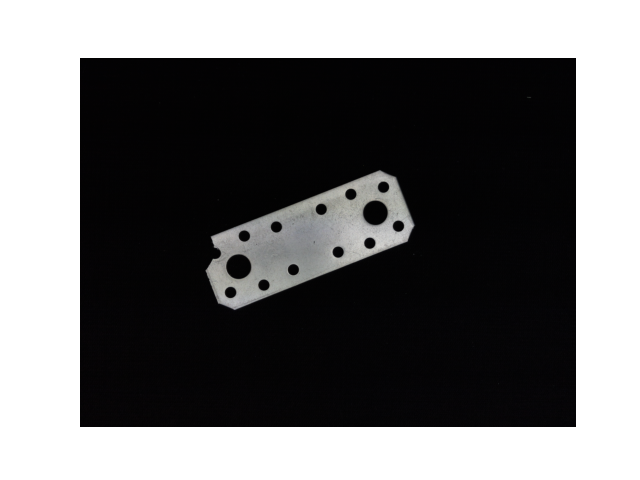
\includegraphics[width=\textwidth]{figures/pca_results/cut_corner.png}
        \caption*{original Image}

    \end{subfigure}
    \begin{subfigure}[b]{0.3\textwidth}
        \centering
        
\includegraphics[width=\textwidth]{figures/pca_results/cut_corner_mask.png}
        \caption*{Mask}

    \end{subfigure}
    \begin{subfigure}[b]{0.3\textwidth}
        \centering
        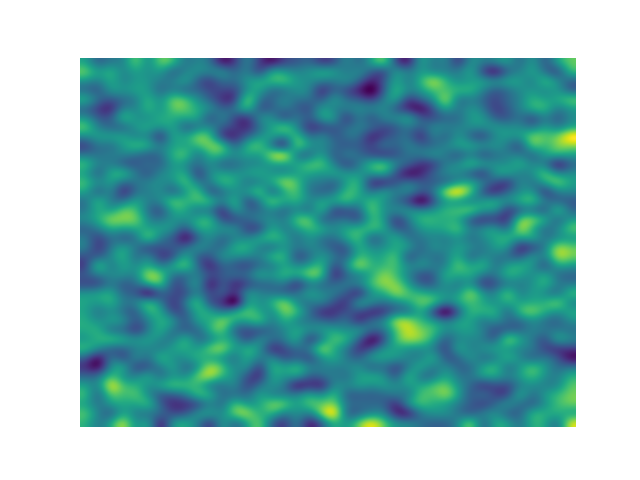
\includegraphics[width=\textwidth]{figures/pca_results/pca_res.png}
        \caption*{Discriminator Predictions}

    \end{subfigure}
    \caption{Results of Independent Transformation Block Ensembles Section \ref{sec:featurelevelensemble}}
    \label{fig:pca_res}
\end{figure}

As visible in figure \ref{fig:pca_res}, the segmentation results appeared to be not more meaningful than gaussian noise, strongly suggesting that this method has failed. Subsection 
\ref{subsec:ITBfaildiscussion} will go into possible reasons for the suboptimal experiments results. Concludingly it is to be said that these results are, besides the failure analysis 
in the conclusion, not relevant and will not be part of further review. Thus no results of other classes using this method are posted in the appendix.

\subsection{Stacking Ensemble}
\label{subsec:stacking}
This subsection reports the performance of both ensemble experiments with stacking as the ensemble method. 
The experiment is split into two smaller experiments. One investigates the performance of ensembling higher and lower level features in 
single backbones, wheras the other one regards standard backbone ensembling with the ones mentioned in section \ref{sec:ensemblecandidates}. 

- table mit metrics


\textbf{Hierarchy Levels.} The results of ensembling different hierarchies exhibit a degree of diversity between different layer hierarchies. As briefly menitoned in section \ref{sec:ensemblecandidates}, the resnet backbones consist of four 
layers, in other words they contain four larger sequential blocks. Inference using higher level feature representations with an backbone of subtype resnet resulted in unusable results, segmentation wise. 
Figure xyz exemplary showcases the segmentation results of training using the wideresnet50 backbone and including a feature aggregation between layers 3 and 4. 



\begin{figure}[htbp]
    \centering
    \begin{subfigure}[b]{0.45\textwidth}
        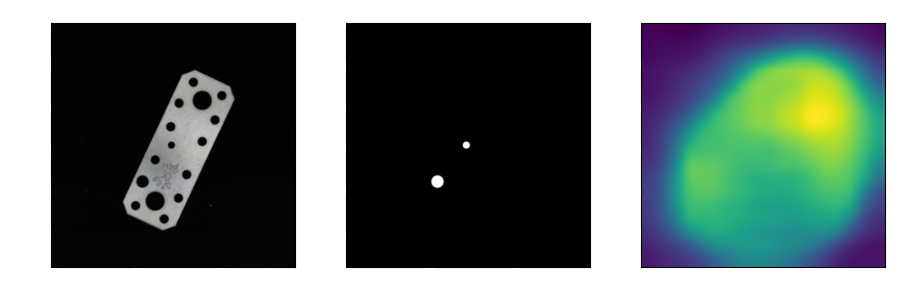
\includegraphics[width=\textwidth]{figures/faillayer34/flat_connector_test_logical_anomalies_001.png}

    \end{subfigure}
    \begin{subfigure}[b]{0.45\textwidth}
        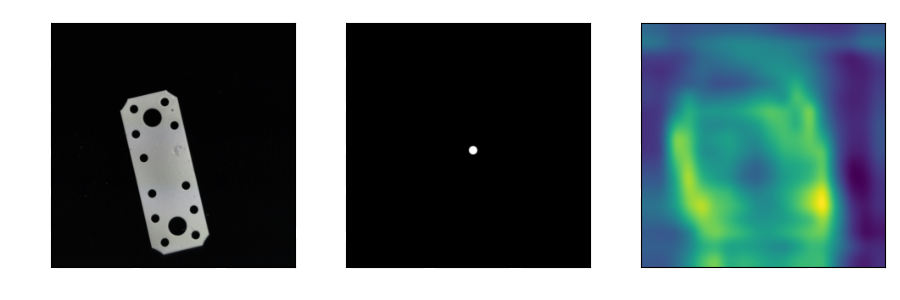
\includegraphics[width=\textwidth]{figures/faillayer34/flat_connector_test_logical_anomalies_023.png}

    \end{subfigure}
    \caption{Resulting segmentations of ensemble network training when utilizing layer 4.}
    \label{fig:faillayersegments}
\end{figure}

The image and pixel AUROC were unstable and poor over the course of the training, 
as figure xyz suggests, and therefore were not recorded explicitly for multiple classes, as this was the case for all trainings. The loss visible in figure xyz furthermore 
showcases that the training process was flawed. Due to these findings the following experiments only consider earlier layers if diverging from the standard layers 
discussed in section \ref{sec:ensemblecandidates}.

\begin{figure}[htbp]
    \centering
    \begin{subfigure}[b]{0.4\textwidth}
        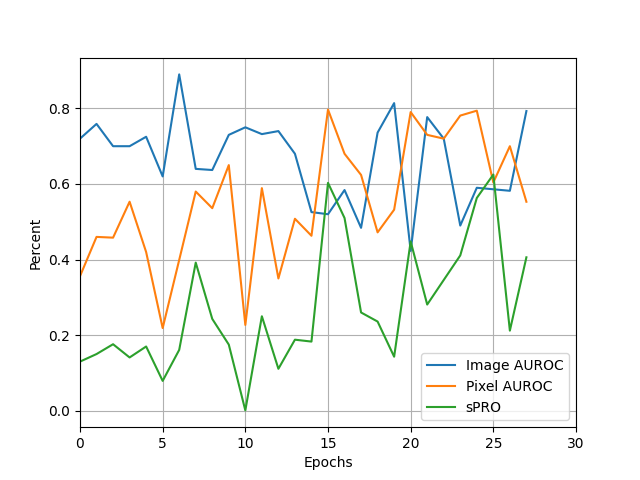
\includegraphics[width=\textwidth]{figures/faillayer34/auprosetc.png}
        \caption{Testing metrics over the course of 30 meta epochs. Usually may contain fluctuations, but not of this amplitude.}
        \label{fig:failmetrics}
    \end{subfigure}
    \begin{subfigure}[b]{0.4\textwidth}
        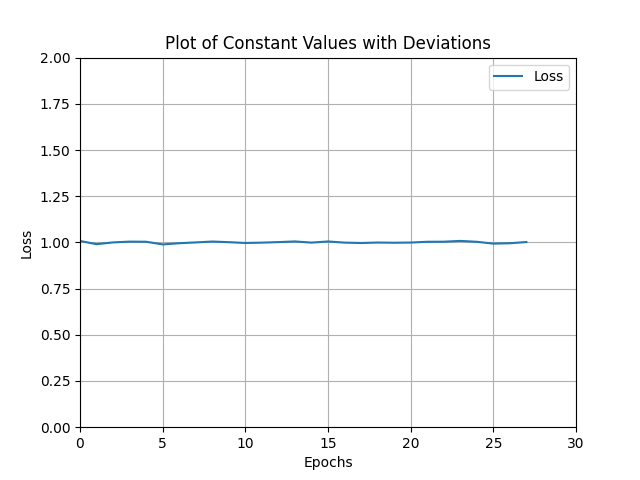
\includegraphics[width=\textwidth]{figures/faillayer34/loss_fail.png}
        \caption{The networks loss during 30 meta epochs. Shows only very little deviations from value 1, not desirable behavior.}
        \label{fig:failloss}
    \end{subfigure}
    \caption{Training metrics and loss of ensemble network training, utilizing layer 4.}
    \label{fig:failmetricsloss}
\end{figure}



Experiments combining lower layer aggregations yielded different results. Table xyz summarises the reported metrics on the flat connector class, and figure xyz showcases exemplary 
segmentation images of the experiments. More data is to be found in the appendix.

- figures hier


\textbf{Backbone Ensemble.} The performance of this approach is visible in table xyz. The performance is visible worse from the performance 
reported by the standard simplenet approach. Yet the results suggest usable results unlike the experiment conducted in section \ref{subsec:ITBfail}. 
Moreover the loss, presented in figure xyz, suggests a conceptually adequate learning. The performance could not be increased by a higher 
epoch count as to be seen by the loss progression in the other subfigure.

- loss figure

Moreover figure xyz showcases exemplary segmentation results on the flat connector class. As 
seen the ensemble ouputs consist of a lot more uncertainty, as the values are closer together and visually harder to distinguish This uncertainty 
was higher for logical anomalies than for structural ones. Still, 
using threshoolding the results are usable, as often anomalous regions are discernible. Figure xyz also showcases examples of failed segmentation 
attempts. 

- figure mit segments 

As a comparison figure xyz displays example segmentations from the individual backbones. Here there is a lot less uncertainty or 
noise than in the ensembled approach. This makes for worse or at least more unstable ensemble performance, especially regarding segmentation. 
The implications and reasons of this are taken up in the next chapter.




